\documentclass[a4paper]{article}
\usepackage[utf8]{inputenc}
\usepackage[russian,english]{babel}
\usepackage[T2A]{fontenc}
\usepackage[left=10mm, top=20mm, right=18mm, bottom=15mm, footskip=10mm]{geometry}
\usepackage{indentfirst}
\usepackage{amsmath,amssymb}
\usepackage[italicdiff]{physics}
\usepackage{graphicx}
\graphicspath{{images/}}
\DeclareGraphicsExtensions{.pdf,.png,.jpg}
\usepackage{wrapfig}
\usepackage{float}
\usepackage{subcaption}
\usepackage{enumitem}
\usepackage{pdflscape}
\usepackage{caption}
\usepackage{array}
\captionsetup[figure]{name=Рисунок}
\captionsetup[table]{name=Таблица}

\title{\underline{Отчет о выполненой лабораторной работе 5.4.2}}
\author{Воронин Денис, Б04-407}

\begin{document}

\maketitle

\begin{center}
\textbf{\Large Исследование энергетического спектра $\beta$ - частиц и определение их максимальной энергии при помощи магнитного спектрометра}
\end{center}

\textbf{Цель работы:} С помощью магнитного спектрометра исследуется энергетический спектр $\beta$-частиц при распаде ядер ${}^{137}\mathrm{Cs}$ и определяется их максимальная энергия. Калибровка спектрометра осуществляется по энергии электронов внутренней конверсии ${}^{137}\mathrm{Cs}$.

\textbf{В работе используются:} источник бета частиц, диафрагма, магнитная линза, свинцовый фильтр, входное окно счетчика.

\section{Аннотация}

По окончании работы должны будем измерить фон, прокалибровать спектрометр, построить график Ферми - Кюри и по этому графику определить максимальную энергию в бета спектре.

\section{Теоретические сведения}

Радиоактивность - явление самопроизвольного распада ядер с испусканием одной или нескольких частиц. Такие ядра называются радиоактивными. \par

Радиоактивный распад характеризуется: временем протекания, сортом испускаемых частиц, энергией, угловой корелляцией. \par

Исходное ядро называется родительским, а продукт дочерним. \par

Виды: $\alpha$, $\beta$, $\gamma$, K - захват, деление ядер.\par

$\textbf{$\alpha$ - распад}$: \par

происходит в тяжелых атомах z > 83, A = 140 - 160 \par

Должна быть энергетическая выгода: \[
\Delta E = E_{A-4, Z-2} + E_\alpha - E_{A, Z} > 0.
\]

Энергия связи альфа частицы = 28 МэВ\par

Проницаемость барьера: 

\[
\begin{aligned}
\ln D \simeq \frac{2\sqrt{2m_\alpha}}{\hbar} \int_{R_\alpha}^{R_{\text{n}}} \sqrt{\frac{2(Z-2)e^2}{r}} \, dr &= -\text{const} \cdot \int_{R_\alpha}^{R_{\text{n}}} \frac{dr}{\sqrt{r}} \simeq \\
&\simeq -(A\sqrt{R_{\text{n}}} - B) = -A \left( \frac{B}{\sqrt{E}} + C \right),
\end{aligned}
\]

Закон Гейгера - Нэттола: \[
\lg T_{1/2} = \frac{a}{\sqrt{E}} + b,
\]

Константа распада:

\[
\lambda = \frac{\ln 2}{T_{1/2}} = \nu D.
\]

$\textbf{$\beta$ - распад}$: \par

Бета - распад - процесс самопроизвольного вревращения нестабильного ядра в ядро - изобар(A - одинаковое и z = +-1)\par
\newpage
\begin{figure}[!hb]
	\centering
	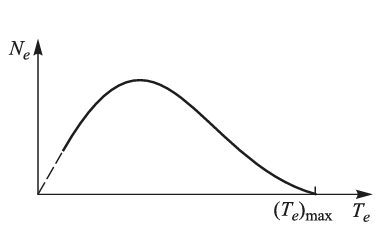
\includegraphics[width=0.3\linewidth]{p1.png}
	\caption{Бета спектр - расперделение числа вылетающих частиц по энергии}
	\label{pic_2}
\end{figure}

Спектр бета распада непрерывный (из-за нейтрино)

\begin{figure}[!hb]
	\centering
	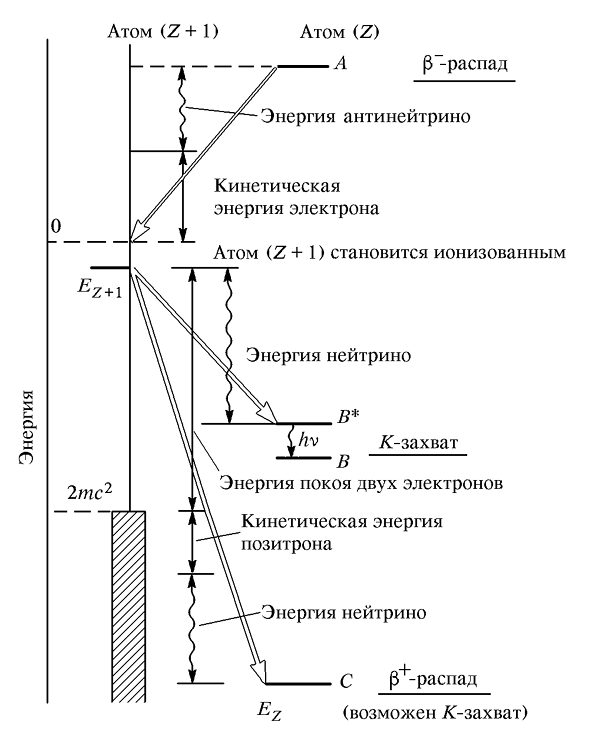
\includegraphics[width=0.3\linewidth]{p2.png}
	\caption{Энергетическая схема бета - распада}
	\label{pic_2}
\end{figure}

Электронный распад связан с распадом нейтрона:
\[
n^0 \to p^+ + e^- + \tilde{\nu}.
\]

При позитронном распаде в ядре распадается протон:
\[
p^+ \to n^0 + e^+ + \nu.
\]

$\textbf{$\gamma$ - распад}$: \par

Гамма - излучение происходит, когда невозможен распад ядра с вылетом нуклона то есть, происходит снитие аозбуждения за счет испускания гамма квантов. (100 кэВ)\par

Гамма - излучение обуславливает взаимодейтсивие нуклонного ядра с э-м полем. \par

Гамма - излучение явление внутриядерное\par

Правмла отбора: 1) закон сохранения четности волновой фукции\par

2) \[
|I_{\text{н}} - I_{\text{к}}| \leqslant L \leqslant I_{\text{н}} + I_{\text{к}}.
\]

В работе будем иметь дело с электронным распадом:

\[
{}^{A}_{Z}\mathrm{X} \to {}^{A}_{Z+1}\mathrm{X} + e^{-} + \tilde{\nu},
\]

Вероятность бета распада равна стат весу \par

Связь кин эн электронов и импульса: 

\[
E = c\sqrt{p^2 + m^2c^2} - mc^2,
\]

Дочерние ядра, возникающие в результате $\beta$-распада, нередко оказываются возбужденными. Возбужденные ядра отдают свою энергию либо излучая $\gamma$-квант (энергия которого равна разности энергий начального и конечного уровней), либо передавая избыток энергии одному из электронов с внутренних оболочек атома. Излучаемые в таком процессе электроны имеют строго определенную энергию и называются $\textbf{конверсионными}$.

% \begin{figure}[!hb]
% 	\centering
% 	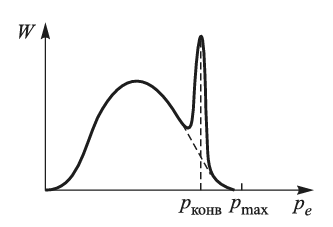
\includegraphics[width=0.3\linewidth]{p3.png}
% 	\caption{Форма спектра бета частиц при разрешенных переходах}
% 	\label{pic_2}
% \end{figure}

Тонкая катушка эквивалентна линзе. Ее фокусное расстояние:

\[
\frac{1}{f} \propto \frac{I^2}{p_e^2}.
\]

\newpage

\begin{figure}[!hb]
	\centering
	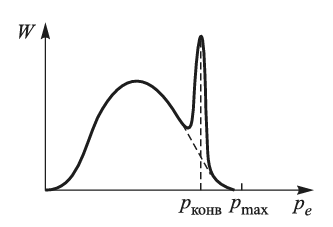
\includegraphics[width=0.3\linewidth]{p3.png}
	\caption{Форма спектра бета частиц при разрешенных переходах}
	\label{pic_2}
\end{figure}

Импульс сфокусированных электронов:

\[
p_e = kI.
\]

\section{Экспериментальная установка}

\begin{figure}[!hb]
	\centering
	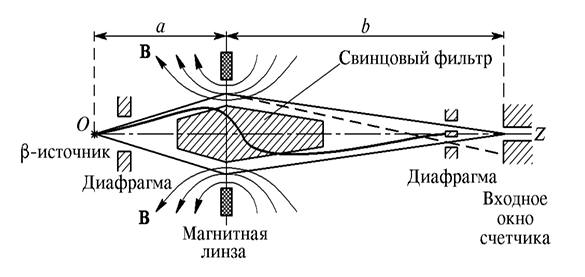
\includegraphics[width=0.5\linewidth]{p4.png}
	\caption{Схема Бета-спектрометра с короткой магнитной линзой}
	\label{pic_2}
\end{figure}

\begin{figure}[!hb]
	\centering
	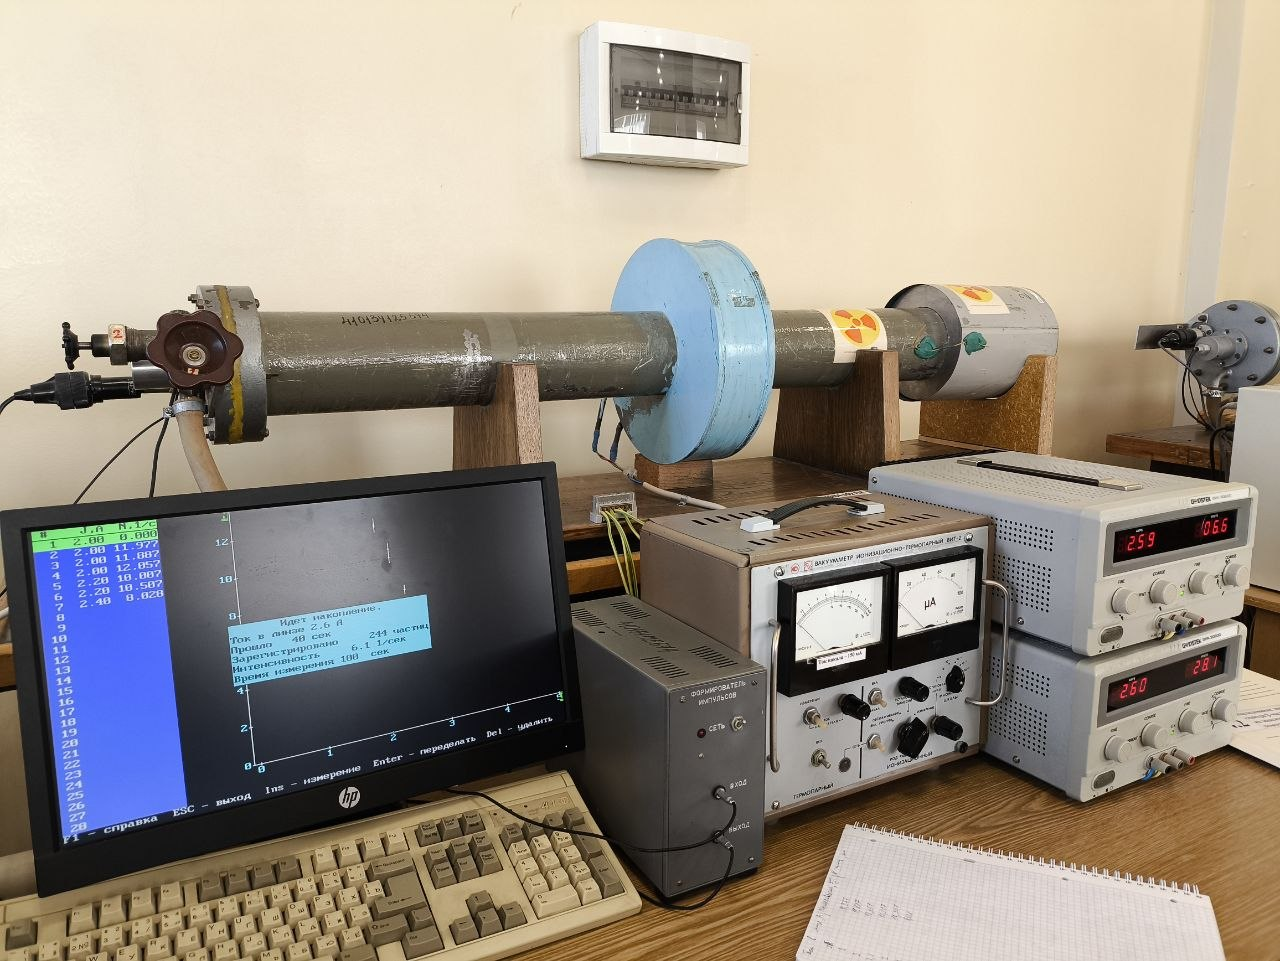
\includegraphics[width=0.5\linewidth]{p1.jpg}
	\caption{Установка}
	\label{pic_2}
\end{figure}

\newpage

\section{Ход работы}

1. Откачаем воздух из установки. Включим вакууметр.\par

2. Включим программу для проведения эксперимента.\par

3. Включим формирователь импульсов, питание магнитной линзы и уменьшим ток через нее до 0.\par

4. Проведем 3 одинаковых измерения с I = 2 А и U = 26,2 В:

\begin{center}
\begin{tabular}{|c|c|}
\hline
\textbf{I, A} & \textbf{N, 1/c} \\
\hline
2 & 11,977 \\
2 & 11,887 \\
2 & 12,057 \\
\hline
\end{tabular}
\end{center}

5. Измерим подробно бета спектр, особенно в области конверсионного пика:

\begin{center}
\begin{tabular}{|c|c|}
\hline
\textbf{I, A} & \textbf{N, 1/c} \\
\hline
2,2 & 10,007 \\
2,4 & 8,028 \\
2,6 & 5,658 \\
2,8 & 3,099 \\
3   & 4,279 \\
3,05 & 8,318 \\
3,1 & 12,036 \\
3,15 & 13,076 \\
3,2 & 15,085 \\
3,25 & 14,026 \\
3,3 & 12,236 \\
3,35 & 11,107 \\
3,4 & 9,467 \\
3,45 & 7,178 \\
3,5 & 4,909 \\
3,6 & 2,399 \\
3,8 & 0,72 \\
4   & 0,6 \\
4,2 & 0,63 \\
4,25 & 0,56 \\
1,8 & 11,946 \\
1,6 & 11,517 \\
1,4 & 9,587 \\
1,2 & 7,478 \\
1   & 4,809 \\
0,8 & 2,349 \\
0,6 & 1,21 \\
0,4 & 1,27 \\
0,2 & 1,14 \\
0,1 & 1,17 \\
0   & 1,24 \\
\hline
\end{tabular}
\end{center}

6. Измерим фон: 0.89 $\frac{1}{c}$

7. Построим график зависимости числа отсчетов от тока:

8. Определим константу прибора: k=316.7 $\frac{\text{кэВ}}{c*A}$

9. Найдем граничную энергию бета спектра по графику Ферми: $T = 610 \pm 35$ кэВ

\newpage

\begin{figure}[!hb]
	\centering
	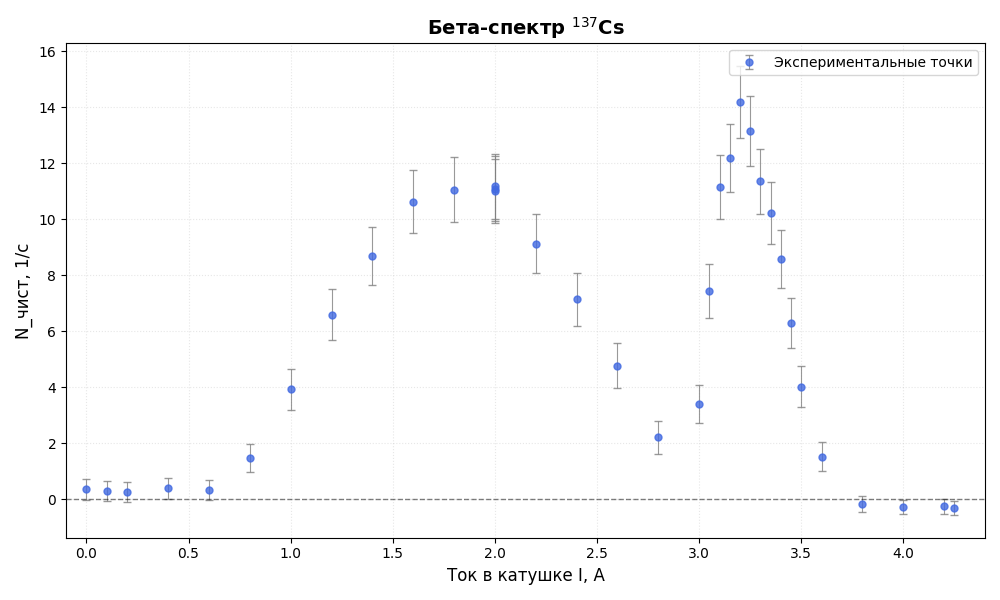
\includegraphics[width=1\linewidth]{F1.png}
	\caption{график зависимости числа отсчетов от тока}
	\label{pic_2}
\end{figure}

\begin{figure}[!hb]
	\centering
	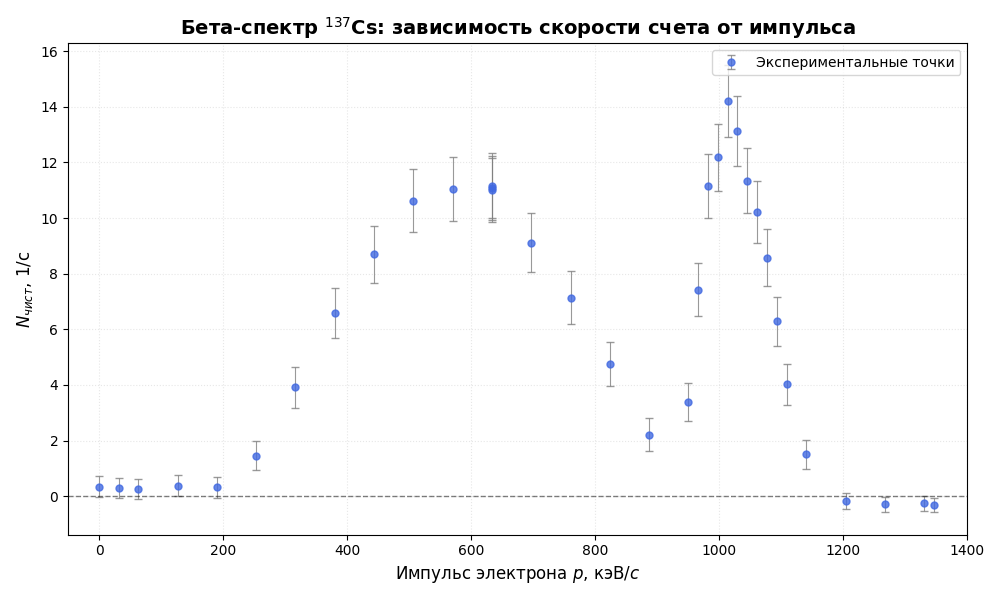
\includegraphics[width=1\linewidth]{F2.png}
	\caption{график зависимости числа отсчетов от импульса}
	\label{pic_2}
\end{figure}
\newpage
\begin{figure}[!hb]
	\centering
	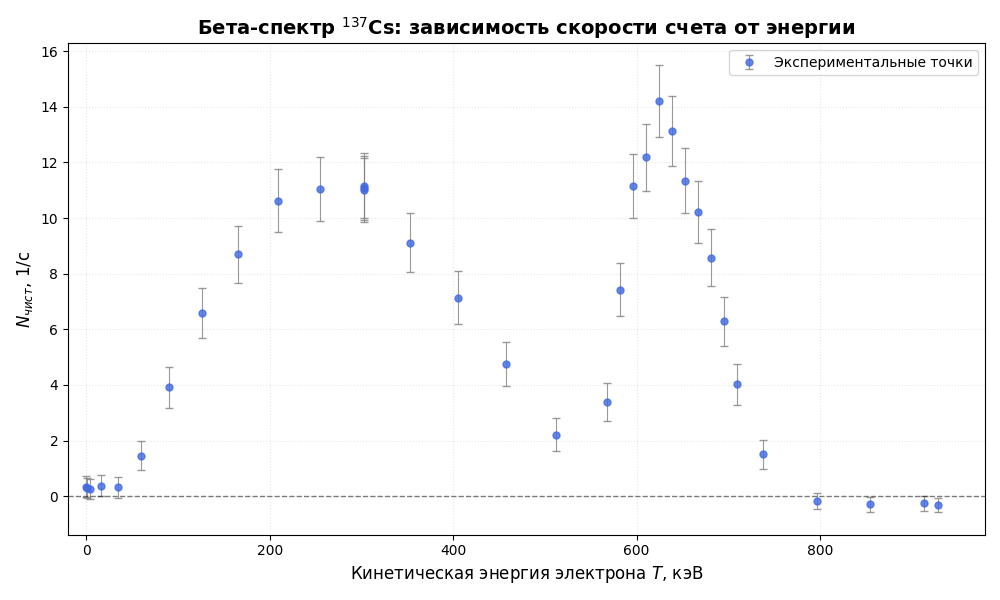
\includegraphics[width=1\linewidth]{F3.png}
	\caption{график зависимости числа отсчетов от кин энергии}
	\label{pic_2}
\end{figure}

\begin{figure}[!hb]
	\centering
	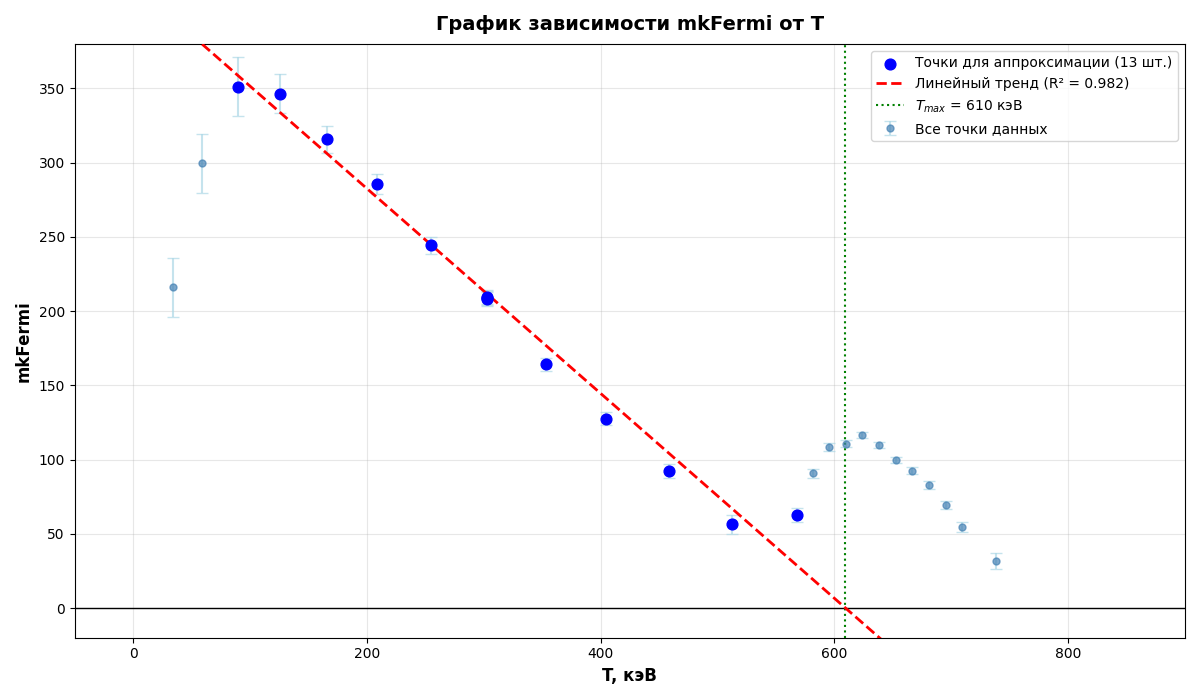
\includegraphics[width=1\linewidth]{F4.png}
	\caption{график зависимости mkfermi от T}
	\label{pic_2}
\end{figure}

\newpage

\section{Вывод}

В ходе лабораторной работы с помощью магнитного спектрометра был исследован энергетический спектр $\beta$-частиц при распаде ядер ${}^{137}\mathrm{Cs}$. При помощи графика Ферми--Кюри была также определена максимальная энергия $T_{\max} = 610 \pm 35$~кэВ вылетающих электронов при $\beta$-распаде ядра ${}^{137}\mathrm{Cs}$. Истинное же значение равно $T_{\max} = 624$~кэВ.

\end{document}